\documentclass[aspectratio=169,12pt]{beamer}
\usepackage{amsmath}
\usepackage{amssymb}
\usepackage[most]{tcolorbox}
\usepackage{tikz}
\usepackage{graphicx}
\usepackage[sfdefault,lf]{FiraSans}
\renewcommand{\familydefault}{\sfdefault}
\setlength{\parindent}{0pt}
\everymath{\displaystyle}

\setbeamertemplate{navigation symbols}{}
\setbeamertemplate{footline}{}
\setbeamertemplate{headline}{}

\definecolor{mmpageWhite}{HTML}{FCFBF7}
\definecolor{mmtanSoft}{HTML}{F7F5EF}
\definecolor{mmgreenDeep}{HTML}{244B2C}
\definecolor{mmgreenLeaf}{HTML}{5D8A56}
\definecolor{mmgreenSoft}{HTML}{E4EFD9}
\definecolor{mmtext}{HTML}{163221}

\setbeamercolor{background canvas}{bg=mmpageWhite}
\setbeamercolor{normal text}{fg=mmtext,bg=mmpageWhite}

\newtcolorbox{MMProblemCard}[1][]{enhanced,breakable=false,colback=white,colframe=black,boxrule=1.0pt,arc=5pt,left=3pt,right=3pt,top=2pt,bottom=2pt,before skip=0pt,after skip=0pt,height=0.26\textheight,valign=top,#1}
\newcommand{\KoruIcon}{\raisebox{-0.2em}{
\includegraphics[height=1.05em]{../../SITE/header-logo.png}}}
\newcommand{\HoeIcon}{\raisebox{-0.2em}{
\includegraphics[height=1.05em]{../../SITE/hoe.png}}}
\newcommand{\ScaffoldIcons}[1]{\ifcase#1\or \HoeIcon\or \HoeIcon\hspace{0.22em}\KoruIcon\or \KoruIcon\hspace{0.22em}\KoruIcon\hspace{0.22em}\KoruIcon\fi}
\newcommand{\WorksheetTitle}[2]{%
  {\colorbox{mmtanSoft}{\parbox[c][2.0em][c]{0.975\linewidth}{%
    \hspace{0.25em}{\Large\bfseries\textcolor{mmgreenDeep}{#1}\hfill\ScaffoldIcons{#2}}}}
  \par\vspace{0.08em}{\color{mmgreenLeaf}\rule{\linewidth}{2.0pt}}\par\vspace{0.04em}}
}
\newcommand{\MMProblem}[2]{\begin{MMProblemCard}\raggedright\small\textbf{#1.} #2\par\end{MMProblemCard}}

\setbeamertemplate{background}{
 \begin{tikzpicture}[remember picture,overlay]
 \draw[black,line width=1.5pt,rounded corners=10pt]
 ([xshift=0.45cm,yshift=-0.45cm]current page.north west)
 rectangle
 ([xshift=-0.45cm,yshift=0.45cm]current page.south east);
 \end{tikzpicture}
}

% Default worksheet generation rules:
% use notes-style beamer pages
% use bordered cards for individual problems
% target 9 problems per frame in a 3x3 grid
% target 3 frames per scaffold by default where content allows

\begin{document}\begin{frame}[t]
\WorksheetTitle{Push Tasks}
\vspace{-0.18em}
\begin{columns}[T,onlytextwidth]
\begin{column}{0.32\textwidth}\MMProblem{1}{The scatter plot shows the relationship between hours studied and test score (out of 100). Describe the relationship using TARSOG.\\[0.4em]
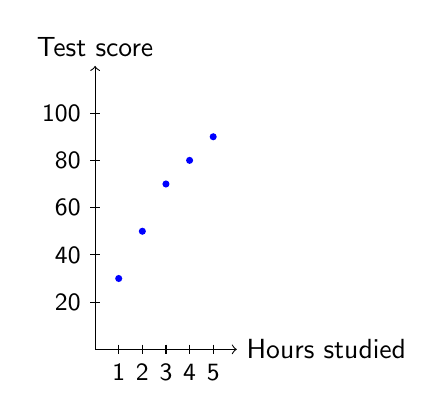
\begin{tikzpicture}[x=0.3cm,y=0.3cm,baseline=(current bounding box.center)]
  \draw[->] (0,0) -- (6,0) node[right] {Hours studied};
  \draw[->] (0,0) -- (0,12) node[above] {Test score};
  \foreach \x in {1,...,5} \draw (\x,0.2) -- (\x,-0.2) node[below] {\small \x};
  \foreach \y in {20,40,60,80,100} \draw (0.2,\y/10) -- (-0.2,\y/10) node[left] {\small \y};
  \fill[blue] (1,3) circle (0.15);
  \fill[blue] (2,5) circle (0.15);
  \fill[blue] (3,7) circle (0.15);
  \fill[blue] (4,8) circle (0.15);
  \fill[blue] (5,9) circle (0.15);
\end{tikzpicture}}\end{column}
\begin{column}{0.32\textwidth}\MMProblem{2}{The scatter plot shows the relationship between temperature (°C) and ice cream sales. Describe the relationship using TARSOG.\\[0.4em]
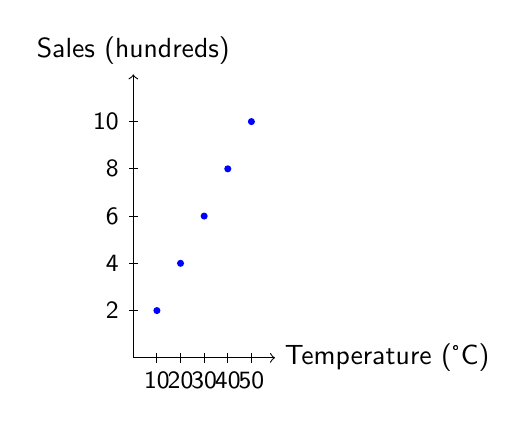
\begin{tikzpicture}[x=0.3cm,y=0.3cm,baseline=(current bounding box.center)]
  \draw[->] (0,0) -- (6,0) node[right] {Temperature (°C)};
  \draw[->] (0,0) -- (0,12) node[above] {Sales (hundreds)};
  \foreach \x in {10,20,30,40,50} \draw (\x/10,0.2) -- (\x/10,-0.2) node[below] {\small \x};
  \foreach \y in {2,4,6,8,10} \draw (0.2,\y) -- (-0.2,\y) node[left] {\small \y};
  \fill[blue] (1,2) circle (0.15);
  \fill[blue] (2,4) circle (0.15);
  \fill[blue] (3,6) circle (0.15);
  \fill[blue] (4,8) circle (0.15);
  \fill[blue] (5,10) circle (0.15);
\end{tikzpicture}}\end{column}
\begin{column}{0.32\textwidth}\MMProblem{3}{The scatter plot shows the relationship between age of a car and its resale value. Describe the relationship using TARSOG.\\[0.4em]
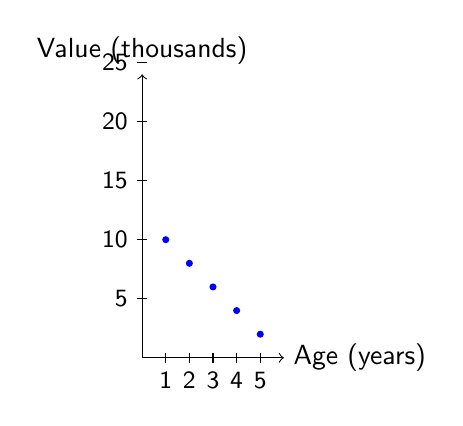
\begin{tikzpicture}[x=0.3cm,y=0.3cm,baseline=(current bounding box.center)]
  \draw[->] (0,0) -- (6,0) node[right] {Age (years)};
  \draw[->] (0,0) -- (0,12) node[above] {Value (thousands)};
  \foreach \x in {1,...,5} \draw (\x,0.2) -- (\x,-0.2) node[below] {\small \x};
  \foreach \y in {5,10,15,20,25} \draw (0.2,\y/2) -- (-0.2,\y/2) node[left] {\small \y};
  \fill[blue] (1,5) circle (0.15);
  \fill[blue] (2,4) circle (0.15);
  \fill[blue] (3,3) circle (0.15);
  \fill[blue] (4,2) circle (0.15);
  \fill[blue] (5,1) circle (0.15);
\end{tikzpicture}}\end{column}
\end{columns}
\vspace{0.45em}
\begin{columns}[T,onlytextwidth]
\begin{column}{0.32\textwidth}\MMProblem{4}{Write a statistical paragraph for each of the three scatter plots above, using TARSOG to describe the relationship.}\end{column}
\begin{column}{0.32\textwidth}\MMProblem{5}{For the first scatter plot, predict the test score for a student who studied 6 hours. Explain your reasoning.}\end{column}
\begin{column}{0.32\textwidth}\MMProblem{6}{For the second scatter plot, predict ice cream sales on a 25°C day. Explain your reasoning.}\end{column}
\end{columns}
\vspace{0.45em}
\begin{columns}[T,onlytextwidth]
\begin{column}{0.32\textwidth}\MMProblem{7}{For the third scatter plot, predict the resale value of a 6-year-old car. Explain your reasoning.}\end{column}
\begin{column}{0.32\textwidth}\MMProblem{8}{Identify any potential outliers in the scatter plots above and discuss how they might affect the interpretation.}\end{column}
\begin{column}{0.32\textwidth}\MMProblem{9}{Identify any groupings in the scatter plots above and suggest possible reasons for the groupings.}\end{column}
\end{columns}
\end{frame}
\begin{frame}[t]
\WorksheetTitle{Push Tasks}
\vspace{-0.18em}
\begin{columns}[T,onlytextwidth]
\begin{column}{0.32\textwidth}\MMProblem{1}{Discuss whether the relationships shown are likely to be causal or merely correlational.}\end{column}
\begin{column}{0.32\textwidth}\MMProblem{2}{Explain how you could collect data to create a scatter plot for a given bivariate relationship.}\end{column}
\begin{column}{0.32\textwidth}\MMProblem{3}{Explain the limitations of using scatter plots to analyse bivariate relationships.}\end{column}
\end{columns}
\vspace{0.45em}
\begin{columns}[T,onlytextwidth]
\begin{column}{0.32\textwidth}\MMProblem{4}{Describe a real-world situation where a scatter plot would be useful, and what TARSOG aspects you would look for.}\end{column}
\begin{column}{0.32\textwidth}\MMProblem{5}{Compare and contrast scatter plots with other statistical displays (e.g., time series graphs, box plots).}\end{column}
\begin{column}{0.32\textwidth}\MMProblem{6}{Explain the importance of considering context when interpreting scatter plots.}\end{column}
\end{columns}
\vspace{0.45em}
\begin{columns}[T,onlytextwidth]
\begin{column}{0.32\textwidth}\MMProblem{7}{Create a sketch of a scatter plot that shows a strong positive linear relationship with constant scatter and no outliers. Label axes appropriately.}\end{column}
\begin{column}{0.32\textwidth}\MMProblem{8}{}\end{column}
\begin{column}{0.32\textwidth}\MMProblem{9}{}\end{column}
\end{columns}
\end{frame}
\end{document}
